\documentclass[10.5pt]{config}
% 本实验报告采用 署名-相同方式共享 4.0 国际许可协议 (CC BY-SA 4.0)
\usepackage{multirow}
\usepackage{wrapfig}
\usepackage{setspace}
\usepackage{titlesec}
\usepackage{ctex}
\usepackage{graphicx} % 用于插入图片
\usepackage{float}    % 用于控制图片位置
\usepackage{makecell}

\titleformat{\subsubsection}[block]  % 设置为块级标题（自动换行）
{\normalfont\bfseries}{\thesubsubsection}{1em}{} 
\titlespacing*{\subsubsection}{1.5em}{3.25ex}{1.5ex}  % 调整缩进：左缩进2em
\setstretch{1.5}

% --- 请在这里填写您的个人信息 ---
\major{机械工程} % 专业
\name{韩颂义}
\partner{} % 签名栏
\stuid{3240104198}
\date{2026年3月26日}
\lab{东三304}
\grades{}
\course{电工电子学实验}
\instructor{季瑞松} % 指导老师
\exptype{验证型} % 实验类型
\expname{MWORKS仿真} % 实验名字


\begin{document}

\makeheader % 首页头部

\section{实验目的和要求（必填）}
% 请在此处填写实验目的和要求

\begin{enumerate}[label=\arabic*., leftmargin=2em]
    \item 掌握 MWORKS 系统仿真软件的图形化操作界面、工作空间构成及基本的仿真流程。
    \item 学习在 MWORKS 环境中搭建基础电工电子电路物理模型的方法，熟练掌握电气元器件模型的调用、参数配置以及信号连线。
    \item 能够正确配置仿真求解器参数并运行仿真，提取关键节点的电压、电流数据，并熟练绘制相关的电气特性曲线（如伏安特性曲线）。
    \item 通过对比仿真测试数据与电工学理论计算结果，探究电压表内阻对电压测量准确度的影响、验证叠加定理、得到二极管的伏安特性曲线。
\end{enumerate}

\section{实验内容和原理}
% 请在此处填写实验内容和原理


\subsection{探究电压表内阻对电压测量准确度的影响}

\textbf{1. 实验原理}

理想的电压表内阻为无穷大，接入电路时不会产生分流作用，从而不影响原电路的工作状态。然而，实际的电压表均存在一定的内阻 $R_V$。当使用实际电压表测量电路中某一电阻 $R$ 两端的电压时，电压表实际上是与该电阻并联。此时，该支路的等效电阻变为：
$$R_{eq} = \frac{R \cdot R_V}{R + R_V}$$
由于 $R_{eq} < R$，接入电压表后改变了电路原有的结构和参数，导致被测节点间的实际电压低于接入电压表前的真实电压。这种由于测量仪器接入而引起的误差称为“负载效应”。只有当 $R_V \gg R$ 时，测量误差才能忽略不计。

\textbf{2. 实验内容}

在 MWORKS 中搭建电路。在被测电阻两端并联一个电阻（模拟实际电压表，万用表阻值约10M$\Omega$，综合实验台上的电压表内阻为500k$\Omega$）。运行仿真，记录不同内阻下的电压测量值，并与理论计算值进行对比，直观观察并分析内阻对测量准确度的影响。

\subsection{验证叠加定理}

\textbf{1. 实验原理}

叠加定理是线性电路分析中的一个重要定理。其内容为：在包含多个独立源（电压源或电流源）的线性电路中，任何一条支路的响应（电流或电压），等于电路中各个独立源单独作用时在该支路所产生的响应的代数和。

当一个独立源单独作用时，其他独立源必须置零：
\begin{itemize}
    \item 理想电压源置零：将其短路（即电压设定为 $0\mathrm{V}$）。
    \item 理想电流源置零：将其开路（即电流设定为 $0\mathrm{A}$）。
\end{itemize}

\textbf{2. 实验内容}

在 MWORKS 中搭建电路，进行仿真。

\subsection{得到二极管的伏安特性曲线}

\textbf{1. 实验原理}

二极管是一种典型的非线性元件，其电流与电压的关系不遵循欧姆定律，而是呈现出单向导电性。
其中，$I_S$ 为反向饱和电流，$U$ 为二极管两端电压，$V_T$ 为热电压（常温下约为 $26\mathrm{mV}$），$n$ 为理想因子。
当正向偏置电压超过一定阈值（如硅管约为 $0.7\mathrm{V}$）时，正向电流急剧增加；当反向偏置时，反向电流极小且基本保持不变（击穿前）。

\textbf{2. 实验内容}

在 MWORKS 中接入一个正弦信号的电源。进行仿真，在xy坐标上绘制出二极管的伏安特性曲线。

\section{主要仪器设备}
安装有MWORKS.Sysplorer的电脑

\section{MOWRKS仿真和结果}

\subsection{探究电压表内阻对电压测量准确度的影响}

按照下图构建电路模型，同时为了模拟电压表内阻，将特定阻值内阻（10M、500k$\Omega$）并联进入。
% 建模截图
\begin{figure}[H]
    \centering
    % 请将此处换成你的图片路径
    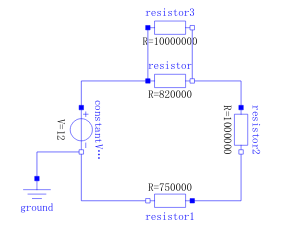
\includegraphics[width=0.6\textwidth, keepaspectratio]{figures/neizu.png}
    \caption{电路建模}
\end{figure}

分别得到万用表、固定电压表（下称电压表）测量时的仿真结果。

% 仿真数据截图
\begin{figure}[H]
    \centering
    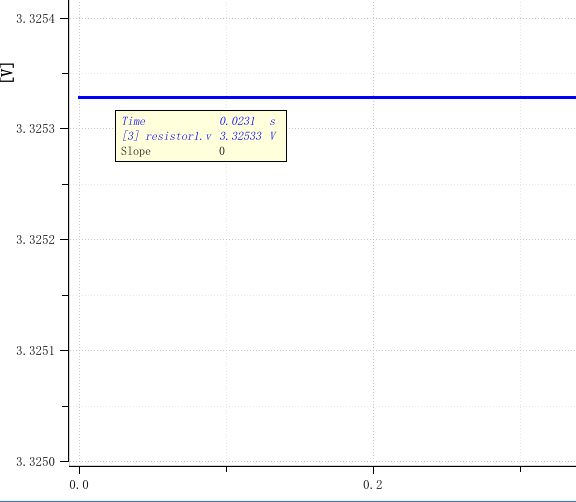
\includegraphics[width=0.6\textwidth, keepaspectratio]{figures/u1.png}
    \caption{万用表接入时U1}
\end{figure}

\begin{figure}[H]
    \centering
    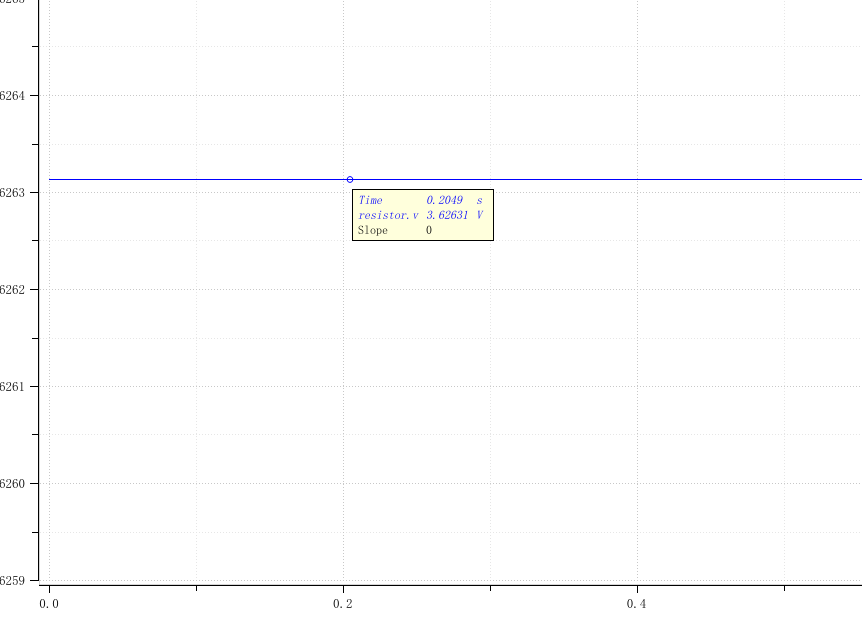
\includegraphics[width=0.6\textwidth, keepaspectratio]{figures/u2.png}
    \caption{万用表接入时U2}
\end{figure}

\begin{figure}[H]
    \centering
    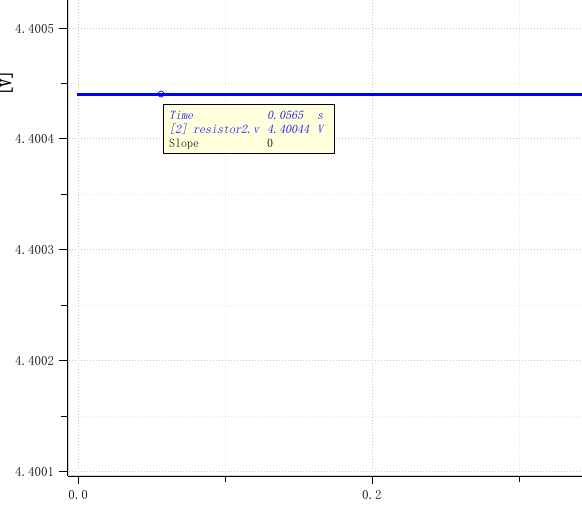
\includegraphics[width=0.6\textwidth, keepaspectratio]{figures/u3.png}
    \caption{万用表接入时U3}
\end{figure}


\begin{figure}[H]
    \centering
    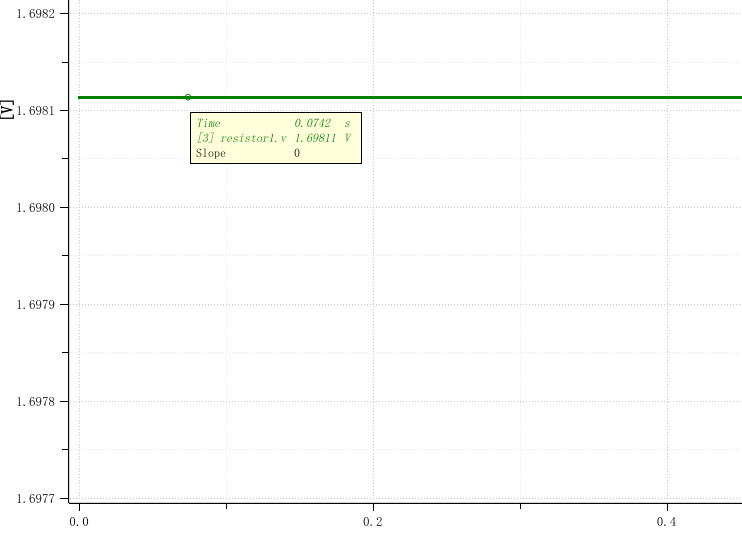
\includegraphics[width=0.6\textwidth, keepaspectratio]{figures/u11.png}
    \caption{电压表接入时U1}
\end{figure}

\begin{figure}[H]
    \centering
    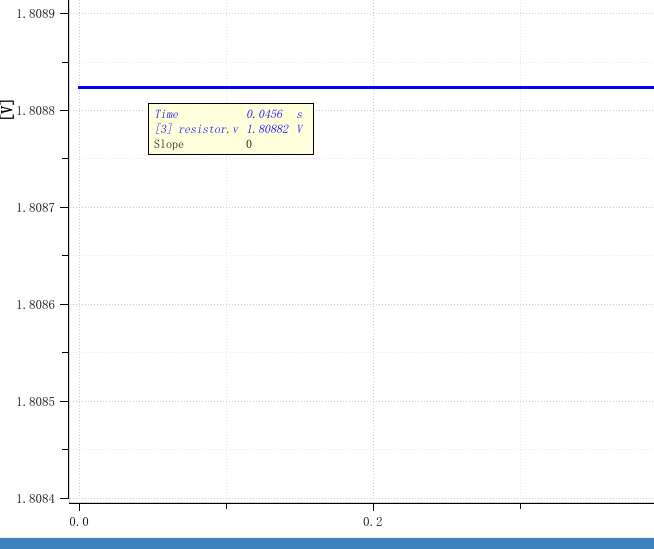
\includegraphics[width=0.6\textwidth, keepaspectratio]{figures/u22.png}
    \caption{电压表接入时U2}
\end{figure}

\begin{figure}[H]
    \centering
    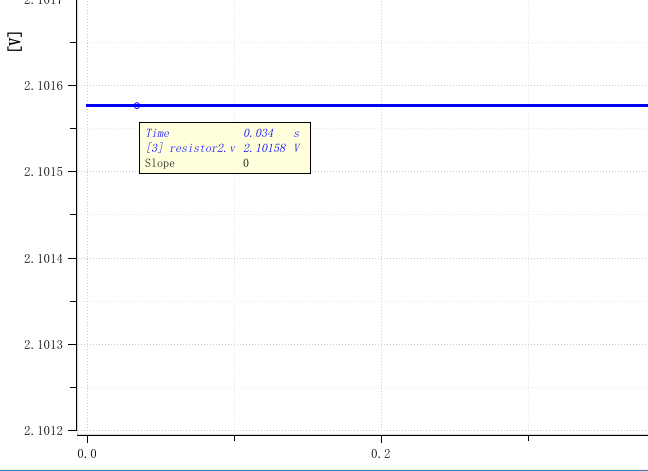
\includegraphics[width=0.6\textwidth, keepaspectratio]{figures/u33.png}
    \caption{电压表接入时U3}
\end{figure}
% 表格中填入仿真数据
\begin{table}[H]
    \centering
    \caption{电压表内阻对电压测量准确度的影响}
    
    \begin{tabular}{|c|c|c|c|c|c|c|c|}
        \hline
        电压表量程 /V & $U_1/\mathrm{V}$ & $U_2/\mathrm{V}$ & $U_3/\mathrm{V}$ & $\Sigma U/\mathrm{V}$（计算）  \\
        \hline
        万用表 20V（或\underline{\hspace{1em}}V）DC &3.32533 &3.62631 &4.40044 &11.35208  \\
        \cline{1-5}
        直流电压表 20V &1.69811 &1.80882 & 2.10158&5.60851 \\
        \hline
    \end{tabular}
    \label{tab:voltmeter_resistance_effect}
\end{table}


\subsection{二极管的伏安特性曲线}

% 建模截图
\begin{figure}[H]
    \centering
    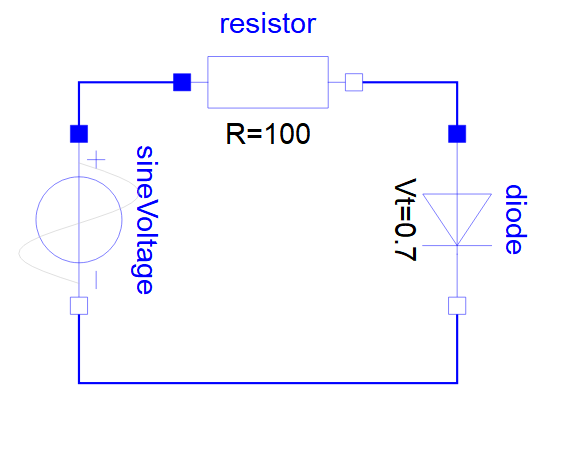
\includegraphics[width=0.6\textwidth, keepaspectratio]{figures/erji.png}
    \caption{二极管电路建模}
\end{figure}

\begin{figure}[H]
    \centering
    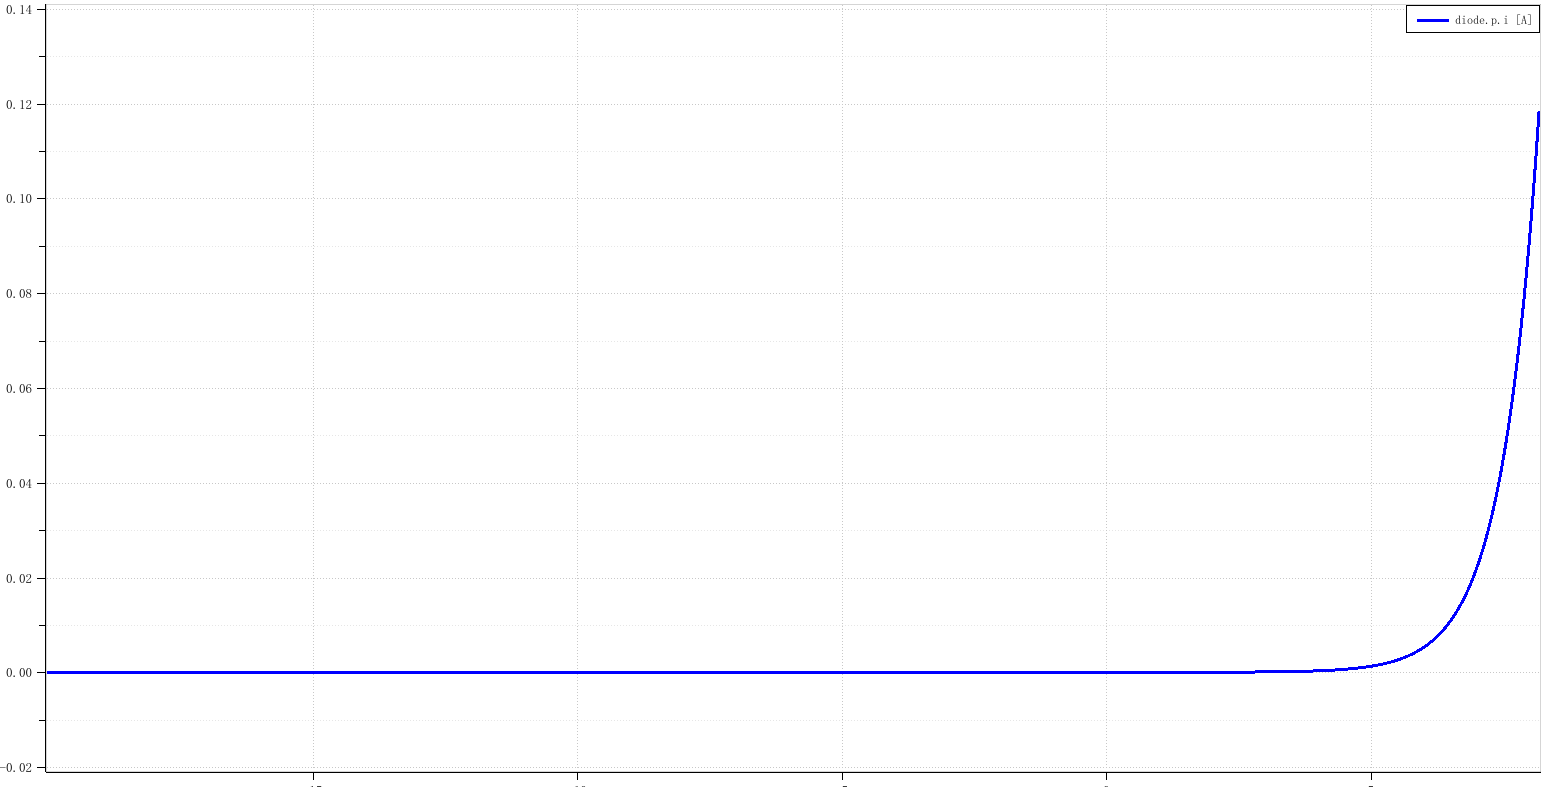
\includegraphics[width=0.6\textwidth, keepaspectratio]{figures/fuan.png}
    \caption{二极管伏安特性曲线}
\end{figure}




\subsection{验证叠加定理}

电压源单独作用

% 建模截图
\begin{figure}[H]
    \centering
    
\includegraphics[width=0.6\textwidth, keepaspectratio]{figures/dianya.png}
    \caption{电压源单独作用}
\end{figure}

得到仿真结果

\begin{figure}[H]
    \centering
    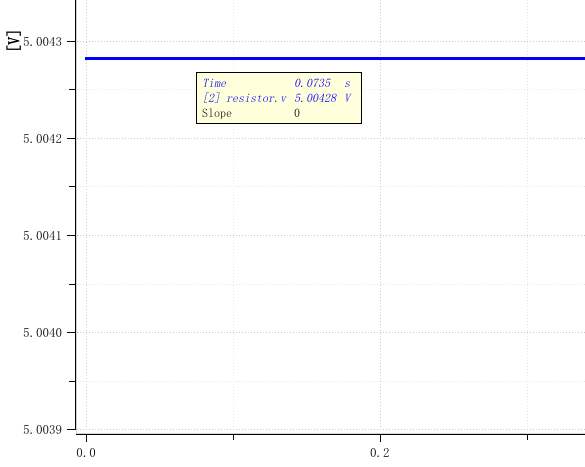
\includegraphics[width=0.6\textwidth, keepaspectratio]{figures/yau1.png}
    \caption{电压源单独作用U1}
\end{figure}

\begin{figure}[H]
    \centering
    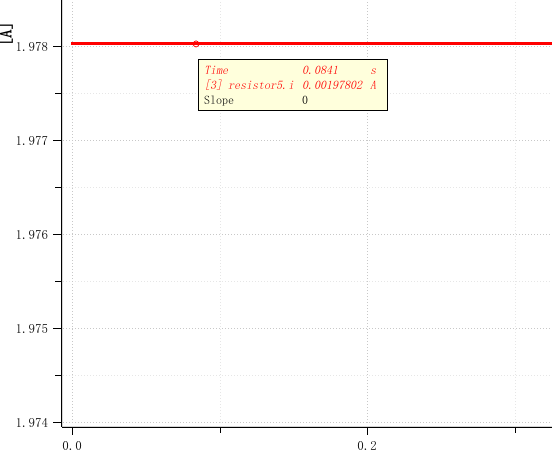
\includegraphics[width=0.6\textwidth, keepaspectratio]{figures/yai2.png}
    \caption{电压源单独作用I2}
\end{figure}

\begin{figure}[H]
    \centering
    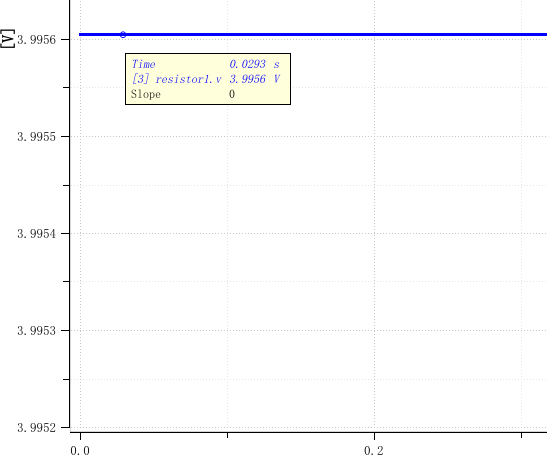
\includegraphics[width=0.6\textwidth, keepaspectratio]{figures/yau3.png}
    \caption{电压源单独作用U3}
\end{figure}



\begin{figure}[H]
    \centering
    
\includegraphics[width=0.6\textwidth, keepaspectratio]{figures/dianliu.png}
    \caption{电流源单独作用}
\end{figure}
\begin{figure}[H]
    \centering
    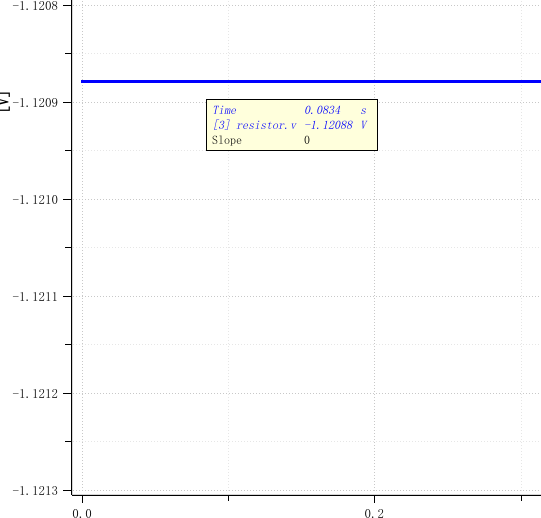
\includegraphics[width=0.6\textwidth, keepaspectratio]{figures/liuu1.png}
    \caption{电流源单独作用U1}
\end{figure}

\begin{figure}[H]
    \centering
    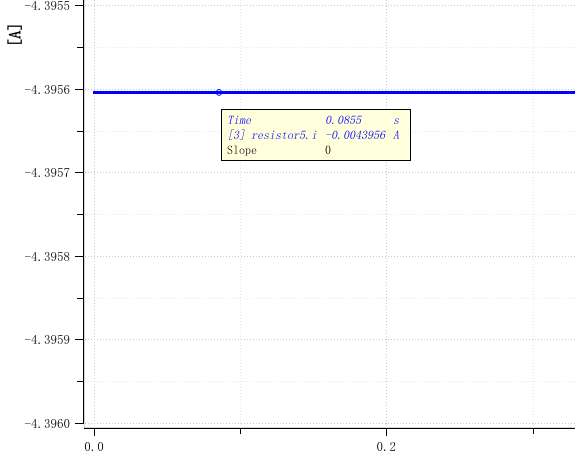
\includegraphics[width=0.6\textwidth, keepaspectratio]{figures/liui2.png}
    \caption{电流源单独作用I2}
\end{figure}

\begin{figure}[H]
    \centering
    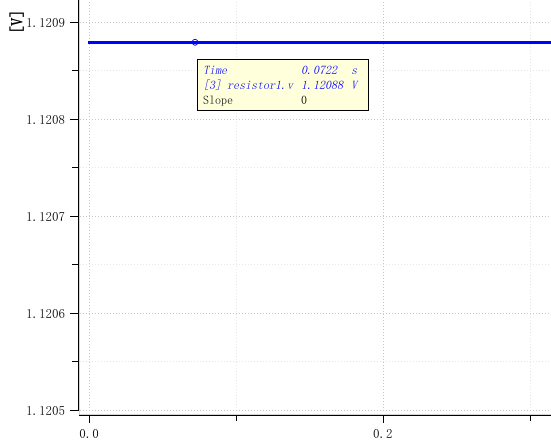
\includegraphics[width=0.6\textwidth, keepaspectratio]{figures/liuu3.png}
    \caption{电流源单独作用U3}
\end{figure}

\begin{figure}[H]
    \centering
    
\includegraphics[width=0.6\textwidth, keepaspectratio]{figures/diejia.png}
    \caption{两者共同作用}
\end{figure}
\begin{figure}[H]
    \centering
    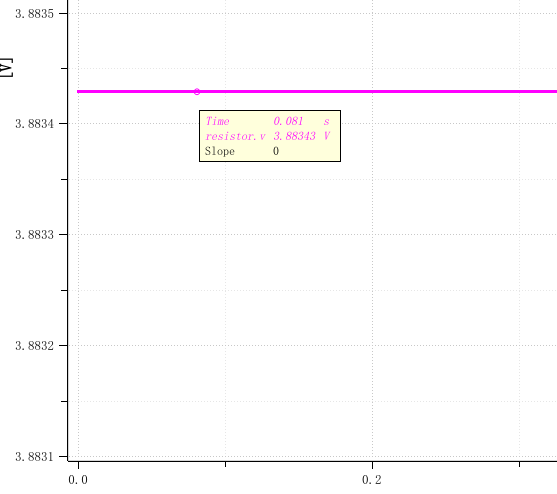
\includegraphics[width=0.6\textwidth, keepaspectratio]{figures/gongu1.png}
    \caption{共同作用U1}
\end{figure}

\begin{figure}[H]
    \centering
    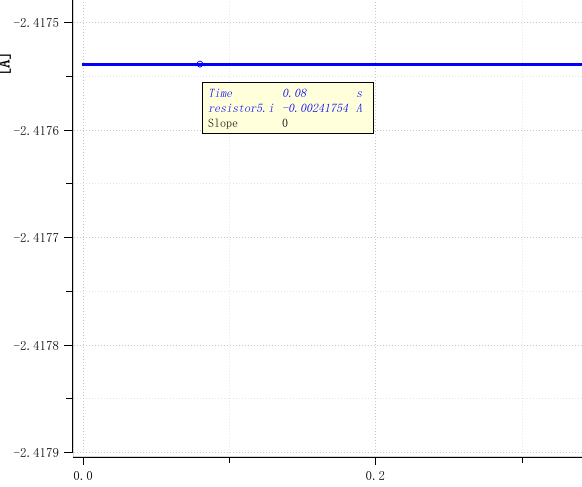
\includegraphics[width=0.6\textwidth, keepaspectratio]{figures/gongi2.png}
    \caption{共同作用I2}
\end{figure}

\begin{figure}[H]
    \centering
    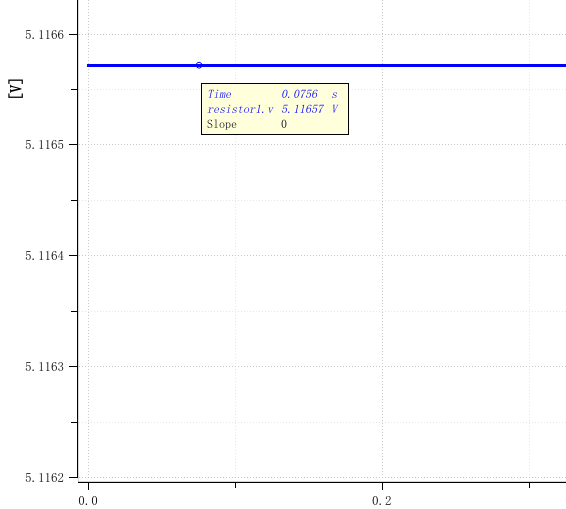
\includegraphics[width=0.6\textwidth, keepaspectratio]{figures/gongu3.png}
    \caption{共同作用U3}
\end{figure}




\begin{table}[H]
    \centering
    \small
    \begin{tabular}{|c|c|c|c|}
        \hline
         & $U_1/\mathrm{V}$ & $I_2/\mathrm{mA}$ & $U_3/\mathrm{V}$ \\
        \hline
        电压源 $U_S$ 单独作用 & 5.00428 & 1.97802 & 3.9956 \\
        \hline
        电流源 $I_S$ 单独作用 & -1.12088 & -4.3956 & 1.12088 \\
        \hline
        以上两者叠加结果（计算） & 3.88340 & -2.41758 & 5.11648 \\
        \hline
        电压源 $U_S$ 与电流源 $I_S$ 共同作用 & 3.88343 & -2.41754 & 5.11657 \\
        \hline
    \end{tabular}
    \caption{验证叠加定理}
    \label{tab:superposn}
\end{table}



\section{实验数据记录和处理}
% 请在此处填写实验数据记录和处理

\section{实验结果与分析（必填）}
% 请在此处填写实验结果与分析

\subsection{电压表内阻对电压测量准确度的影响分析}
根据表 \ref{tab:voltmeter_resistance_effect} 的仿真数据可以看出，当使用模拟内阻为 $10\mathrm{M}\Omega$ 的万用表进行分压测量时，测得的 $U_1$、$U_2$、$U_3$ 之和为 $11.35208\mathrm{V}$；而当使用模拟内阻仅为 $500\mathrm{k}\Omega$ 的直流电压表测量时，三次测量的电压之和骤降至 $5.60851\mathrm{V}$。
\textbf{分析：}这直观地展示了仪表的“负载效应”。当电压表并联在被测电阻两端时，电压表内阻与被测电阻形成并联关系。直流电压表的内阻（$500\mathrm{k}\Omega$）相对较小，其分流作用不可忽略，导致并联后的等效电阻显著减小，从而使该部分分得的实际电压大幅降低。相反，万用表的内阻（$10\mathrm{M}\Omega$）极大，分流作用微弱，测量值更接近真实值。因此，在进行高阻值电路的电压测量时，必须选择高内阻的电压表以减小系统误差。

\subsection{二极管伏安特性分析}
观察仿真输出的二极管伏安特性曲线（图8），可以发现曲线呈现明显的非线性特征。
\textbf{分析：}在正向偏置区域，当电压较小（未达到死区电压）时，正向电流极小，几乎为零；当正向电压超过一定阈值（开启电压）后，曲线变得非常陡峭，电流随电压的微小增加而呈指数级剧增。

\subsection{叠加定理验证分析}
根据表 \ref{tab:superposn} 的数据，将“电压源单独作用”与“电流源单独作用”时的各支路响应（电压和电流）进行代数相加，计算得到叠加结果为：$U_1 = 3.88340\mathrm{V}$，$I_2 = -2.41758\mathrm{mA}$，$U_3 = 5.11648\mathrm{V}$。
将其与“两者共同作用”时的系统仿真结果（$U_1 = 3.88343\mathrm{V}$，$I_2 = -2.41754\mathrm{mA}$，$U_3 = 5.11657\mathrm{V}$）进行对比，可以发现两组数据高度一致，绝对误差在 $10^{-4}$ 数量级。

% 注：原 doc 文档中序号跳过了七直接到了“八、讨论、心得”，这里为你修正为标准编号，或者按照你原模板的习惯使用带有 * 号的 section
\section*{七、讨论、心得}
% 请在此处填写讨论与心得

通过本次 MWORKS 的仿真实验，我收获颇丰，不仅熟悉了系统仿真软件的操作，更对电工学的基础理论有了更具象的认识。

首先，MWORKS 提供了一个极佳的“数字孪生”环境。以往在纸面上推导基尔霍夫定律和叠加定理时，面对的只是干瘪的数学符号和公式；而在物理实验中，又常常受到连线接触不良、仪表损坏等繁杂因素的干扰。利用 MWORKS 进行物理建模，既屏蔽了不必要的硬件干扰，又比纯数学计算更贴近物理本质，让我能专注于电路拓扑和元器件特性本身。

\end{document}